\documentclass[a4paper,11pt]{bgwork}

% Referencing and more
\usepackage[british]{babel}
\usepackage{csquotes}
\usepackage[style=apa,backend=biber]{biblatex}

% Lorem Ipsum
\usepackage{lipsum}

\usepackage[dvips]{hyperref}

% For full width tables
\usepackage{tabularx}

% Images
\usepackage{graphicx}
\graphicspath{ {./images/} }

% Spacing between paragraphs
\usepackage{parskip}

% Section colours
\author{Jacob Sánchez}
\title{Background and Related Work}
\date{17/10/2022}

\addbibresource{References.bib}


\begin{document}

\section{Background and Related Work}
\subsection{Introduction}

Each of your chapters should have an introduction to tell your readers what they will find in the chapter. Eventually this submission will form Chapter 2 of your report, so when you include it in your report it will be numbered accordingly and make sense in context of the whole. It will help you if you create a plan for your report now, with headings and sub-headings, so that you have an idea of your structure and how this chapter fits into the whole.

In this chapter you should summarise current knowledge and what others have done in the various topics of your project – in the application area and in the various technologies that you might have used or did use. You should evaluate that knowledge and state how it is useful for your project Write for someone familiar with computing, but not necessarily expert in the particular topics of your project. Give references to other work by using cross-references to entries in the References section, like this \parencite{turner2002rules}.

It is often useful to start this chapter with an overview of its contents, giving the reasoning behind why you have structured it in a particular way. The main thrust of the chapter is a review of relevant work by other authors and the relationship between this and your own work.

You are aiming for around 8-10 pages for this chapter.

For editorial consistency, it is important to use Word styles properly. If the styles referred to below are not visible on the Home ribbon in the Styles category, choose ‘Apply Styles’ from the down arrow at the bottom right of the Styles category. Styles can then be applied from the drop-down box. To make a style visible as a quick style, choose Apply Styles, then click Styles (the AA icon) or use ‘Alt + Ctrl + Shift + S’, then right-click on the style and then ‘Add to Style Gallery’.

Chapters are entered using the ‘Heading 1’ paragraph style. The Heading 1 style automatically moves to the start of a new page and supplies the next chapter number. Pressing enter on a ‘Heading 1’ heading automatically inserts a ‘Heading 2’ heading underneath.

There should not be any text between a parent heading and its first sub-heading. For example, when you want to write an introductory section for the following sections, give that introductory section an own ‘Introduction’ heading instead of writing it between the heading preceding these sections and the first sub-heading.

Most text uses the ‘Normal Project Body’ paragraph style.

In general, use the default spacing that headings and paragraphs give you. Avoid using new-lines or spaces to format text. If you need to use quotes, preferably use single curly quotes ‘…’. If you wish to emphasise something, use the ‘Emphasis’ style. In addition, also a ‘Strong’ style is preconfigured.

Remember to Save frequently while you are working! Check that AutoSaving is enabled under options -> save -> 'Save AutoRecover information every 5 minutes'.

\subsection{Section Title Rename Me}
\subsubsection{Subsection Title Rename Me}
You may wish to think about theming this chapter. Generally, 3 or 4 themes are enough. State your themes in the introduction and why they are relevant to your project. Each section could correlate to each of your themes. You must remember to state in each section why what you have discussed is relevant to your project, or why you have considered but are discarding it.

Linking your background reading to your project will get you extra marks. This whole chapter needs to link to what you are doing. If you cannot answer the question ‘SO WHAT?’ to everything you include here. then it has no place in this chapter.

You need to be critical and not descriptive, if all you are doing is regurgitating what you read, without being critical and without linking it to your project, you will not get a good mark. Look at the video on Blackboard that covers how to form an argument, it will help you write this chapter.

\subsection{Section Title Rename Me}
\subsubsection{Subsection Title Rename Me}
As an example of a figure, consider Figure \ref{fig:diagram}.

To place a figure, insert the picture / diagram / etc... where you want it to be, make sure it is selected and then apply the ‘Project Figure Title’ style which centres the figure horizontally.

Captions are entered through the ribbon menu under ‘References’ -> ‘Insert Caption’ or through right-clicking an image and selecting ‘Insert Caption’. Add the caption text in the box, separated with a dash as the example below shows.

Each figure is numbered automatically, and it is possible to make cross-references to figures.


\begin{figure}[h]
\centering
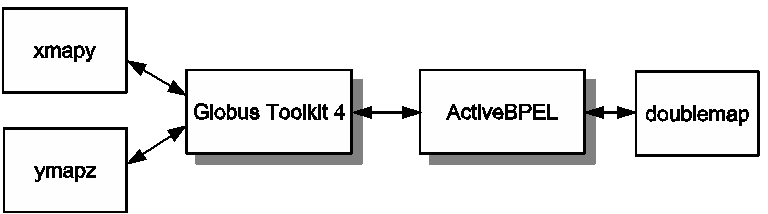
\includegraphics{diagram}
\caption{Highly Technical Diagram}
\label{fig:diagram}
\end{figure}

\subsection{Section Title Rename Me}
\subsubsection{Another Subsection Title Rename Me}

To add a caption to a table, either select the whole table (e.g. by clicking on the + symbol in the upper left corner of the table), right-click it and choose ‘Insert Caption’ or click in any table cell and select ‘References’ -> ‘Insert Caption’ from the ribbon menu. Choose ‘Table’ as label and ‘above the item’ as position. Add the caption text in the box, separated with a dash as the example below shows.


\begin{table}[h]
\begin{tabular}{|l|l|l|l|}
    \hline
    Table Heading 1 & Table Heading 2 & Table Heading 3 & Table Heading 4\\
    \hline
    & & &\\
    \hline
    & & &\\
    \hline
    & & &\\
    \hline
\end{tabular}
\caption{Test Results}

\end{table}

\subsection{Summary}
Write a short summary at the end of this chapter. This is not your conclusions, that will go at the end of your report. This is a summary of the chapter. Have a look at the examples on Blackboard. Do not start this section with ‘In summary’, it is obvious from the heading what it is.

Once you have finished this chapter put it aside for at least 48 hours, then come back to it. READ IT OUT LOUD to yourself, this is a good editing technique.

Then, ask someone else to read it for you.

Get some information feedback from your supervisory team. Make sure you do this with plenty of time before the submission date.


\section*{References}
Use APA styling for your references. Note that this heading is not numbered. Please make sure you use the correct formatting for your references. Despite covering this topic multiple times, many students are still doing it incorrectly. If you are copying and pasting from somewhere else, check that the colour, font face and font size match the style for this document.

You should aim for at least 10-15 references (15 for a 1st). Ensure that the MAJORITY of these are good quality journal papers. This means at least 75\% of them.

\url{https://www.mendeley.com/guides/apa-citation-guide}

\printbibliography
\end{document}
